\documentclass[journal,transmag]{IEEEtran}

\usepackage{}
%\usepackage[pdftex]{graphicx}
% declare the path(s) where your graphic files are

%\graphicspath{IMAGES/}
%\DeclareGraphicsExtensions{.pdf,.jpeg,.png,.jpg}
\usepackage{graphicx}
\usepackage{amsmath}
\interdisplaylinepenalty=2500
\usepackage{algorithmic}
\usepackage{array}
\usepackage[caption=false,font=normalsize,labelfont=sf,textfon =sf]{subfig}
\usepackage{dblfloatfix}
\usepackage{url}
\usepackage{lipsum}
\usepackage{xcolor}
\usepackage{listings}

\lstset{
	escapeinside={/*@}{@*/},
	language=Java,	
	basicstyle=\fontsize{8.5}{12}\selectfont,
	numbers=left,
	numbersep=2pt,    
	xleftmargin=2pt,
	frame=tb,
	columns=fullflexible,
	showstringspaces=false,
	tabsize=4,
	keepspaces=true,
	showtabs=false,
	showspaces=false,
	morekeywords={inline,public,class,private,protected,struct},
	captionpos=b,
	lineskip=-0.4em,
	aboveskip=10pt,
	extendedchars=true,
	breaklines=true,
	prebreak = \raisebox{0ex}[0ex][0ex]{\ensuremath{\hookleftarrow}},
	keywordstyle=\color[rgb]{0,0,1},
	commentstyle=\color[rgb]{0.133,0.545,0.133},
	stringstyle=\color[rgb]{0.627,0.126,0.941},
}

% correct bad hyphenation here
%\hyphenation{-ing}

\begin{document}

\title{Optimising a genetic algorithm using parallelization}

\author{\IEEEauthorblockN{Emils Pinkis, 40122269\IEEEauthorrefmark{1}}
\IEEEauthorblockA{\IEEEauthorrefmark{1}School of Computing,
Edinburgh Napier University, Edinburgh}% <-this % stops an unwanted space

\thanks{}}


%\markboth{What a fucking fantastic header}{}
% The only time the second header will appear is for the odd numbered pages after the title page when using the twoside option.

\IEEEtitleabstractindextext{
\begin{abstract}
    This is an abstract.
\end{abstract}

\begin{IEEEkeywords}
    Napier, what(), \LaTeX, OpenMP, multithreading.
\end{IEEEkeywords}}

\maketitle

\IEEEdisplaynontitleabstractindextext

\IEEEpeerreviewmaketitle

\section{Introduction}
 
\IEEEPARstart{F}{uck}, this is a template for IEEE transaction reports. \textsc{This bit of text is different.} \LaTeX\ is dead, I don't think anyone actually uses it, and we are all being strung along on a terrible joke.

\section{Introduction}}
	\lipsum[1-2]
	This is how you cite something \cite{mrx05}
	
	\subsection{A subsection}
		\lstinputlisting[caption = A code listing.]{./sourceCode/hello.cpp}
	
\section{Section 2}
	\lipsum[3-5]

\section{Section 3}
	\lipsum[6-8]
	
\section{Section 4}
	\lipsum[9-10]
	
\begin{figure}[!t]
	\centering
	\includegraphics[width= 0.5\textwidth]{images/exampleImage}
	\caption{A frog}
	\label{fig_frog}
\end{figure}

\begin{figure}[!t]
	\centering
	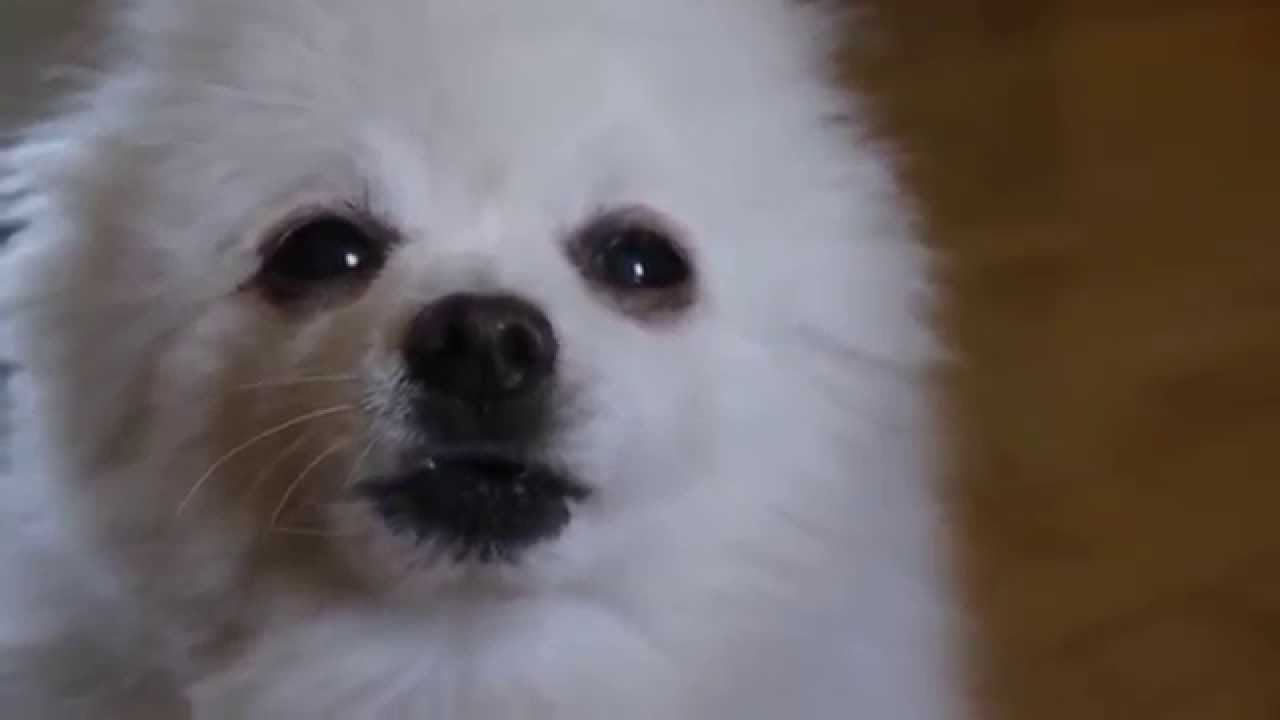
\includegraphics[width= 0.5\textwidth]{images/fig2}
        \caption{A doggo}
	\label{fig_pup}
\end{figure}

\begin{table}[!t]
	\renewcommand{\arraystretch}{1.3}
	\caption{An Example of a Table}
	\label{table_example}
	\centering
	\begin{tabular}{|c|c|}
		\hline
		One & Two\\
		\hline
		Three & tabs\\
		\hline
	\end{tabular}
\end{table}

\section{Conclusion}
The conclusion goes here.

\newpage

\appendices
\section{Proof of something}
	Appendix one text goes here.

\section{}
	Appendix two text goes here.

\section*{Acknowledgement}
	The author would like to thank...

\bibliographystyle{IEEEtran}
\bibliography{bibliography}

\end{document}
